% !TEX root = main.tex

\chapter{Ambiente para el lenguaje de programaci\'on}
\label{chapter.envir}

El programador requiere de una herramienta que le permita ejecutar sistemas distribuidos basados en \SCCP \ modelados en el lenguaje de programaci\'on presentado en el Capi\'tulo~\ref{chapter.lang}. Este cap\'itulo presenta una herramienta desarrollada en Python 3 con una interfaz gr\'afica sencilla y facil de usar, con la que se puede verificar la evaluci\'on de un sistema luego de realizar multiples operaciones de transferencia de informaci\'on entre diferentes agentes. La interpretaci\'on del lenguaje de programaci\'on se realiza por medio de un parser y un analizador l\'exico con los que se genera el codigo equivalente en Maude.  Luego de obtener el estado final del sistema en Maude, se traduce para mostrar el resultado al usuario por medio de la interfaz gr\'afica.

La Secci\'on~\ref{parser.envir} presenta la descripci\'on del parser utilizado en la herramienta. La Secci\'on~\ref{implem.envir} presenta algunos detalles de su implementaci\'on y funcionamiento. La Secci\'on~\ref{gui.envir} presenta una introducci\'on a la interfaz gr\'afica y las funcionalidades de la herramienta. Finalmente, la Secci\'on~\ref{example.envir} presenta algunos ejemplos  pr\'acticos del uso de la herramienta propuesta.

%% Secci\'on:  %%
\section{Parser}
\label{parser.envir}

Cuando se interpreta un lenguaje, es de mucha utilidad usar un un \'arbol de sintaxis concreta (del ingl\'es, \textit{Concrete Syntax Tree}, abreviado CST), tradicionalmente denominados \textit{parse tree}, para representar la estructura sint\'actica del c\'odigo fuente de acuerdo con alguna gram\'atica libre de contexto. Este CST puede ser construido por un parser en el proceso de traducci\'on del codigo fuente y compilaci\'on. 

Un \textit{parser} es un software que a partir de una entrada (i.e. c\'odigo fuente) produce una estructura de datos (i.e. CST o parse tree) basado en una representaci\'on estructural del lenguaje de programaci\'on utilizado para generar la entrada (i.e. EBNF), verificando durante el proceso que la sintaxis sea correcta. El parser es precedido por un analizador l\'exico o \textit{lexer}, el cual crea expresiones o \textit{tokens} a partir de una secuencia de caracteres. 

Sin embrago, construir un parser desde cero es complicado e innecesario debido a que existen multiples herramientas que proveen la construcci\'on del CST de forma automatizada en diferentes lenguajes de programaci\'on, entre ellos Python (v.gr. ANTLR, PyPEG, Parsiomonious).

La herramienta propuesta brinda al programador una interacci\'on sencilla a trav\'es del lenguaje de programaci\'on presentado en el Cap\'itulo~\ref{chapter.lang}, el cual es ejecutado en el fondo en el ambiente de Maude por medio de la especificaci\'on formal del Cap\'itulo~\ref{chapter.rew}, para lograrlo se requiere una traducci\'on por medio de un parser. Para este trabajo se escogio ANTLR~\cite{Parr:2013:DAR:2501720}, un generador parser para leer, procesar, ejecutar y traducir texto estructurado o archivos binarios.

ANTLR genera un parser en Python a partir de la descripci\'on EBNF del lenguaje de programaci\'on, el parser puede construir el \textit{parser tree} de cualquier c\'odigo fuente escrito correctamente en el lenguaje de programaci\'on. Mediante un lexer que se  desarrollado espec\'ificamente para dicho lenguaje se genera el c\'odigo equivalente en Maude. 

%% Secci\'on:  %%
\section{Detalles de la implementaci\'on}
\label{implem.envir}

La herramienta propuesta esta desarrollada en Python 3, un lenguaje de programaci\'on de alto nivel. Debido a que el an\'alisis del sistema \SCCP \ se realiza en Maude, la herramienta provee un enlace entre el parser generado por ANTLR y del ambiente de Maude, a trav\'es del modulo \cde{subprocess} el cual permite crear nuevos procesos y conectarse con su canal de entrada, salida y errores. Este modulo permite ejecutar comandos en la terminal y obtener la salida, tal como se muestra a continuaci\'on: \[\cde{path = subprocess.check_output("pwd",shell=True)},\] en el ejemplo se usa el metodo \cde{subprocess.check_output} para 
ejecutar el comando \cde{pwd} y obtener su resultado, que en este caso es el directorio donde se esta trabajando.

Adicionalmente la herramienta cuenta con una funci\'on que realiza la traducci\'on del estado final del sistema ejecutado en Maude para presentarlo al usuario, en este caso no se utiliz\'o un parser puesto que no se requiere una sintaxis formal para mostrar los resultados.

La herramienta esta divida en dos directorios: Python y Maude. En el primer directorio se encuentran la interfaz gr\'afica, el parser y el lexer; y en el segundo se encuentra la especificaci\'on formal. Su ejecuci\'on se realiza a trav\'es de la linea de comandos.

%% Secci\'on:  %%
\section{Interfaz gr\'afica}
\label{gui.envir}

La interfaz g\'afica de la herramienta esta desarrollada por medio de Tkinter, la libreria mas utilizada para desarrollo de aplicaciones GUI {del ingl\'es, \textit{Graphical User Interface}} en Python. Esta herramienta cuenta con dos ventanas, las cuales se describen en las Figuras~\ref{fig:tool1} y~\ref{fig:tool2}.

\begin{figure}[htbp] %  figure placement: here, top, bottom, or page
   \centering
   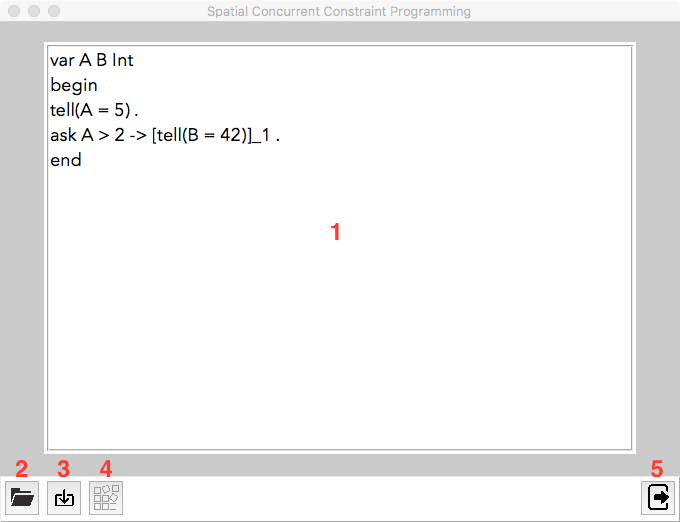
\includegraphics[width=5in]{tool1.png}
   \caption{Ventana principal}
   \label{fig:tool1}
\end{figure}

En la Figura~\ref{fig:tool1} se muestra la ventana principal de la herramienta, donde el programador ingresa el programa o sistema a ejecutar en el lenguaje de programaci\'on propuesto en el Cap\'itulo~\ref{chapter.lang}. Esta ventana cuenta con un editor de texto y una barra inferior con cuatro botones. El editor de texto identificado con el n\'umero \textbf{1}, permite copiar, cortar, pegar y desplazamiento vertical, actualmente no tiene implementado funciones de deshacer y rehacer. La funcionalidad de los botones se explica a continuaci\'on:

\begin{itemize}
\item El boton \textbf{2} permite abrir documentos de texto en formatos \cde{.txt}, \cde{.maude} o \cde{.in}, por medio de una ventana de manejo de archivos. Cuando se selecciona el archivo el contenido se muestra autom\'aticamente en el editor de texto.
\item El boton \textbf{3} permite guardar en un documento texto de formato \cde{.txt}, \cde{.maude} o \cde{.in} el contenido actual del editor de texto, por medio de una ventana de manejo de archivos.
\item El boton \textbf{4} ejecuta el programa escrito en el editor de texto. En caso de que la sintaxis sea incorrecta se muestra un mensaje de error en la ventana de resultados.
\item El boton \textbf{5} permite salir de la herramienta. 
\end{itemize}

\begin{figure}[htbp] %  figure placement: here, top, bottom, or page
   \centering
   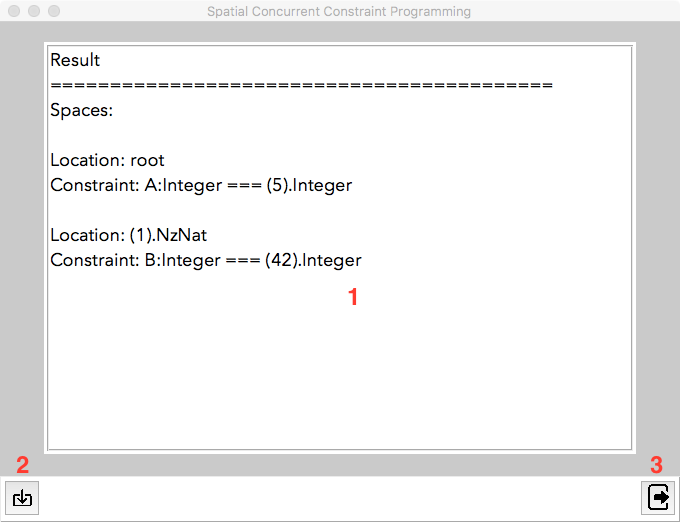
\includegraphics[width=5in]{tool2.png} 
   \caption{Ventana de resultados}
   \label{fig:tool2}
\end{figure}

En la Figura~\ref{fig:tool2} se muestra la ventana de respuestas, en donde se muestra al programador la evoluci\'on del sistema ingresado. Esta ventana cuenta con un cuadro de texto y una barra inferior con dos botones. En el cuadro de texto identificado con el n\'umero \textbf{1} se muestra el resultado de la ejecuci\'on del sistema, en caso de que haya un error en el sistema escrito por el programador se muestra un mensaje correspondiente. El cuadro de texto no permite modificar o seleccionar el texto. Los botones \textbf{2} y \textbf{3} permiten guardar el contenido del texto en un archivo de formato \cde{.txt}, \cde{.maude} o \cde{.out}, y cerrar la ventana de resultados, respectivamente.

En la ventana de respuestas se presenta el estado final del sistema en dos secciones, los agentes existentes y sus respectivos bancos de informaci\'on, y los procesos que no se pudieron ejecutar. 

Las dos ventanas cuentan con un menu desplegable con las mismas funcionalidades explicadas en esta secci\'on. Este cap\'itulo concluye con algunos ejemplos del funcionamiento de la herramienta.

%% Secci\'on:  %%
\section{Ejemplo}
\label{example.envir}

Utilizando la herramienta propuesta en este cap\'itulo se utiliza el ejemplo trabajado en las secciones anteriores para verificar que se llega al esta final deseado a partir del c\'odigo escrito en la Secci\'on~\ref{example.lang}. En la Figura~\ref{fig:toolin1} se muestra el estado incial $d$ junto con el proceso $S$.

\begin{figure}[htbp] %  figure placement: here, top, bottom, or page
   \centering
   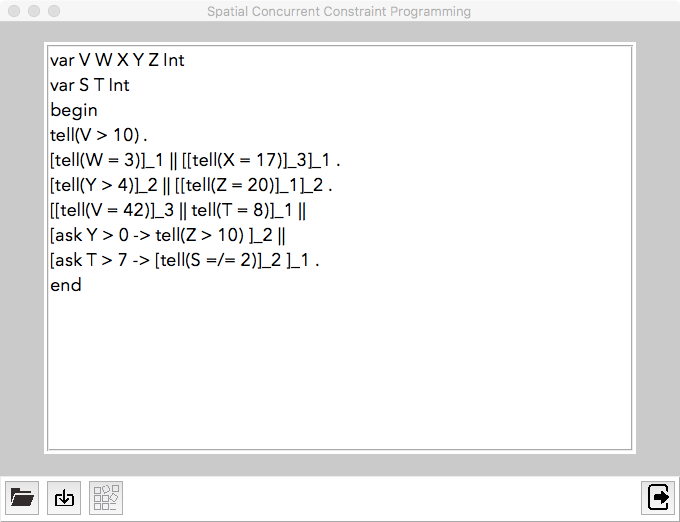
\includegraphics[width=5in]{toolex1.png} 
   \caption{Estado inicial $d$ del sistema}
   \label{fig:toolin1}
\end{figure}

En la Figura~\ref{fig:toolout1} se muestra el estado final del sistema obtenido de la herramienta, el resultado concuerda con el estado final esperado descrito en la Figura~\ref{fig:sccptree2}. En el resultado los agentes (\textit{spaces}) son listados con su identificador (\textit{location}) y su banco de informaci\'on (\textit{constraint}). 

\begin{figure}[htbp] %  figure placement: here, top, bottom, or page
   \centering
   \begin{subfigure}[b]{5in}
      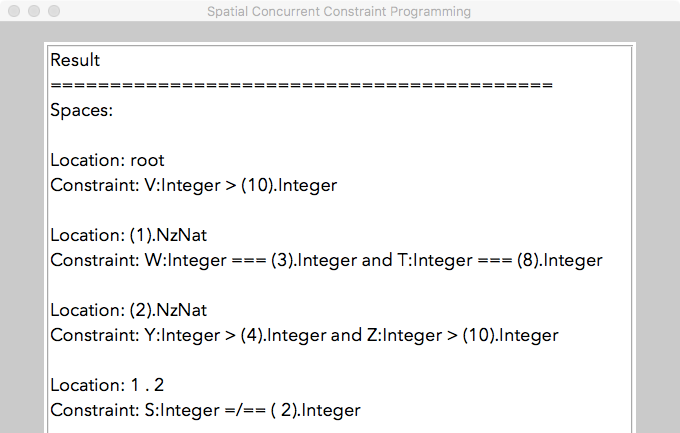
\includegraphics[width=1\linewidth]{toolex2.png}
      \caption{}
      \label{fig:Ng1} 
   \end{subfigure}
   \begin{subfigure}[b]{5in}
      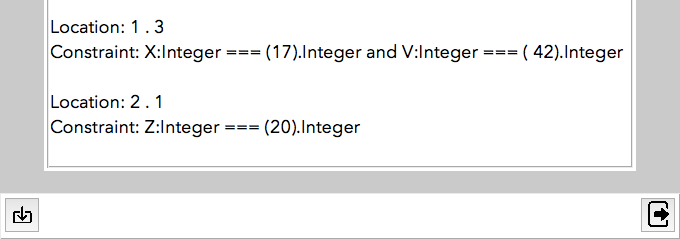
\includegraphics[width=1\linewidth]{toolex22.png}
      \caption{}
      \label{fig:Ng2}
   \end{subfigure}
   \caption{Estado final del sistema}
   \label{fig:toolout1}
\end{figure}

Considere un sistema en el cual no se puede ejecutar un proceso \ask \ debido a que la restricci\'on no es satisfacible por el banco de informaci\'on del agente. En el siguiente ejemplo existen dos procesos que se pueden ejecutar, por lo tanto el sistema no evoluciona y el resultado debe coincidir con su estado inicial. El estado inicial del sistema se describe a continuaci\'on:

\begin{sccp}
var A B C D Int
begin
tell(A =/= 10) .
ask A = 10 -> tell(B >= 5) .
[tell(C > 5) || ask C > 6 -> tell(D = 8)]_1 .
end
\end{sccp}

En la Figura~\ref{fig:toolout3} se observa que existen dos procesos que no fueron ejecutados, el primero de ellos debido a que \cde{A = 10} no es satisfacible a partir de \cde{A =/= 10}. 

\begin{figure}[htbp] %  figure placement: here, top, bottom, or page
   \centering
   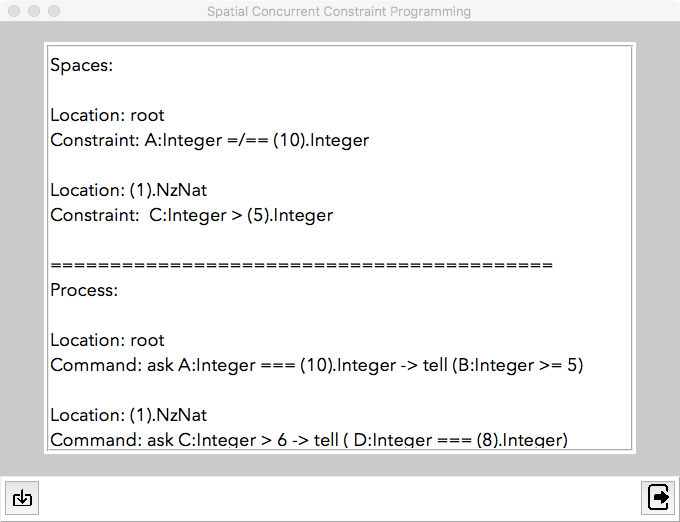
\includegraphics[width=5in]{toolex3.png} 
   \caption{Estado final del sistema con procesos no ejecutados}
   \label{fig:toolout3}
\end{figure}

Finalmente, si el programador no define una variable usada dentro del sistema se genera un mensaje de error, debido a que el lexer no sabe como manejar el token y por lo tanto no se genera la expresi\'on correspondiente. El mensaje ``\cde{Sorry, there is an error!. Check your specification and try again.}'' aparece en la ventada de resultados.


